% vim: tw=80 noai
\documentclass[normaltoc,capchap,capsec,times]{abnt}
\usepackage[utf8x]{inputenc}
\usepackage[T1]{fontenc}
\usepackage[brazil]{babel}
\usepackage[alf]{abntcite}
\usepackage[ordem=alf]{tabela-simbolos}
\usepackage{url}
\usepackage[pdftex]{graphicx}
\usepackage{listings}
\usepackage{verbatim}
\usepackage{subfigure}
\usepackage{multicol}
\usepackage{framed}
\def\lstlistingname{Listagem}

%%%%%%%%%%%%%%%%%%%%%%%%%%%%%%%%%%%%%%%%%%%%%%%%%%%%
% Dados da monografia
%%%%%%%%%%%%%%%%%%%%%%%%%%%%%%%%%%%%%%%%%%%%%%%%%%%%

\newcommand{\meunome}{Aline Duarte Bessa}
\newcommand{\meutitulo}{PROVISORIO: Um estudo sobre \emph{Opinion Mining}}
\newcommand{\meusubtitulo}{PROVISORIO: Aspectos teóricos e práticos}
\newcommand{\meuano}{2010}
\newcommand{\meuorientador}{Orientador: Alexandre Tachard Passos}
\newcommand{\meucoorientador}{Co-orientador: Luciano Porto Barreto}

%%%%%%%%%%%%%%%%%%%%%%%%%%%%%%%%%%%%%%%%%%%%%%%%%%%%

%% O comando \obs aqui definido permite que o autor faca anotacoes na
%% monografia que aparecem no PDF gerado. Para ativar o comando, descomente
%% a primeira linha e comente a segunda.
%% Exemplo de uso: \obs{Preciso melhorar este par�grafo...}

%\newcommand{\obs}[1]{\underline{\textbf{OBSERVAÇÃO}}: \emph{#1}}
\newcommand{\obs}[1]{}

\def\ordfem{\mbox{\raise .35em \hbox{\underline{\scriptsize a}\ }}}
\def\ordmasc{\mbox{\raise .35em \hbox{\underline{\scriptsize o}\ }}}
\def\profa{Prof\ordfem.}

%%%%%%%%%%%%%%%%%%%%%%%%%%%%%%%%%%%%%%%%%%%%%%%%%%%%

\begin{document}

% Capa com Brasão

\begin{titlepage}
   \begin{center}
      %logotipo
               
\includegraphics{brasaoUFBA} \\
  %\vspace{0.7in}
              \centering{ 
        \bf{
        \LARGE{
    \uppercase{UNIVERSIDADE FEDERAL DA BAHIA} \\
        }
        \Large {
                    \uppercase{INSTITUTO DE MATEMÁTICA} \\
        }
                   \large {
                       \uppercase{DEPARTAMENTO DE CIÊNCIA DA COMPUTAÇÃO} \\
                  }
              } }
   \end{center}
   \vfill
   \begin{center}
       \bf{
       \large{\uppercase{\meunome}  \\  }
       }
   \end{center}
   \vspace{0.2in}
   \begin{center}
       \bf{
         \LARGE{ \uppercase{\meutitulo} } \\
         \Large{ \uppercase{\meusubtitulo} }
         \obs{\\ \Large{Esta versão da monografia contém comentários do autor.
          Para removê-los, redefina o comando LaTeX \texttt{obs}.}}
       }
   \end{center}

   \vfill
   \hspace{\stretch{1}}
   \vfill
   \begin{center}
      \normalsize{
          Salvador \\
          \meuano
       }
   \end{center}

\end{titlepage}

%comando abaixo cria uma capa redundante, mas como a capa com brasão foi 
% feita 'manualmente', não faz sentido usar este comando:
%\capa



%\folhaderosto
% o comando acima foi comentado para não criar uma folha de 
% rosto redundante, já que ela feita 'manualmente' abaixo

\begin{titlepage}
 \vfill
 \begin{center}
   {\large \uppercase{ \bf{ \meunome\ } } } \\[7cm]
   {\Huge \uppercase{ \bf{ \meutitulo\ } } }\\[1cm]
   \vfill
   \hspace{.45\textwidth} % posicionando a minipage
   \begin{minipage}{.5\textwidth}
     \begin{espacosimples}
       \bf{
  Monografia apresentada ao Curso de graduação em Ciência da Computação, 
  Departamento de Ciência da Computação, Instituto de Matemática,  Universidade Federal da 
  Bahia, como requisito parcial para obtenção do grau de Bacharel em  Ciência da Computação. \\ 
       }      
     \end{espacosimples}
     \begin{espacosimples}    
       \meuorientador \\
       \meucoorientador
     \end{espacosimples}
   \end{minipage}
   \vfill
   Salvador \\
   \meuano
 \end{center}
\end{titlepage}


\begin{resumo}
Nonono nonono nonono, nonono, nonono nonono nonono nononono nonno.
Nonono nonono nonono, nonono, nonono nonono nonono nononono nonno.
Nonono nonono nonono, nonono, nonono nonono nonono nononono nonno.
Nonono nonono nonono, nonono, nonono nonono nonono nononono nonno.
Nonono nonono nonono, nonono, nonono nonono nonono nononono nonno.
Nonono nonono nonono, nonono, nonono nonono nonono nononono nonno.
Nonono nonono nonono, nonono, nonono nonono nonono nononono nonno.

\textbf{Palavras-chave:}
monografia,
graduação, 
projeto final.
\end{resumo}

% O abstract e' opcional.
\begin{abstract}
Nonono nonono nonono, nonono, nonono nonono nonono nononono nonno.
Nonono nonono nonono, nonono, nonono nonono nonono nononono nonno.
Nonono nonono nonono, nonono, nonono nonono nonono nononono nonno.
Nonono nonono nonono, nonono, nonono nonono nonono nononono nonno.
Nonono nonono nonono, nonono, nonono nonono nonono nononono nonno.
Nonono nonono nonono, nonono, nonono nonono nonono nononono nonno.
Nonono nonono nonono, nonono, nonono nonono nonono nononono nonno.

\textbf{Keywords:} 
monograph,
graduation,
final project.
\end{abstract}

%% As listas a seguir sao opcionais:
\listadefiguras
%\listadetabelas
\listadesiglas
%\listadesimbolos

\sumario

% O conteudo da monografia esta' nos seguintes arquivos:
\chapter{Introdução}

%\section{Motivação}

A busca por opiniões sempre desempenhou um papel importante na geração de novas escolhas. Antes de optar por assistir a um filme, é comum ler críticas a seu respeito ou considerar os comentários de outras pessoas; antes de comprar um produto, muitas vezes procuramos relatos sobre a satisfação de outros consumidores. Com a disseminação da Web e da Internet, a geração de opiniões com impacto, sobre os mais diversos assuntos, foi finalmente democratizada: não é mais preciso, por exemplo, ser um especialista em Economia ou Ciência Política para manter um \emph{blog} convincente sobre algum candidato às eleições.

Neste contexto, a busca por opiniões e comentários em \emph{sites}, \emph{blogs}, fóruns e redes sociais também se popularizou, passando a fazer parte do cotidiano dos consumidores \emph{online}. Uma pesquisa feita nos Estados Unidos revelou que entre 73\% e 87\% dos leitores de resenhas de serviços online, como críticas de restaurantes e albergues, sentem-se fortemente influenciados a consumi-los ou não a depender das opiniões contidas nessas resenhas \cite{pesquisa-eua}. Diante da relevância que opiniões têm na geração de decisões e no processo de consumo, estudos com o intuito de extraí-las da Web e interpretá-las automaticamente tornaram-se mais frequentes na área de Ciência da Computação. Juntos, esses estudos compõem o que ficou conhecido como \textbf{Análise de Sentimento} ou \textbf{Mineração de Opinião}, termos utilizados como sinônimos \cite{omsa} \cite{bingliu}.

De acordo com a \emph{survey} de Pang e Lee, referência mais citada para o estudo da área, a Mineração de Opinião envolve o emprego de diversas técnicas computacionais com o intuito de explorar algum dos tópicos abaixo \cite{omsa}:

\begin{enumerate}
    \item \textbf{Polaridade de sentimento ou graus de polaridade -} Dado um documento opinativo, para o qual se assume que as opiniões se referem basicamente a um único assunto, classifique-o como positivo ou negativo em relação a esse assunto (polaridades opostas) ou localize-o no espectro estabelecido entre duas polaridades opostas;
    \item \textbf{Detecção de subjetividade e identificação de opinião -} Dado um documento, detecte se ele é subjetivo ou não, constituindo-se de fatos ou opiniões, ou que partes dele são subjetivas;
    \item \textbf{Análise de tópico-sentimento -} Dado um documento opinativo, assume-se que suas opiniões podem se referir a tópicos diferentes, e deve-se identificar quais opiniões interagem com quais tópicos;
   \item \textbf{Pontos de vista ou perspectivas -} Dado um documento opinativo, que apresente uma perspectiva sobre um tema (um ponto de vista, uma orientação ideológica, um posicionamento), em vez de um sentimento polarizado sobre um único assunto, classifique-o de acordo com essa perspectiva;
   \item \textbf{Outras informações não-factuais -} Dado um documento com caráter emotivo/sentimental, identifique que tipos de humor o permeiam e/ou classifique-o de acordo com as emoções encontradas.

\end{enumerate}

O item \textbf{Pontos de vista ou perspectivas}, em particular, é de grande aplicabilidade para as Ciências Humanas. Diferentemente dos outros tópicos, mais aplicáveis à compreensão de opiniões \textbf{pontuais} sobre marcas/produtos/pessoas públicas, esse item investiga um fenômeno mais profundo: o posicionamento\footnote{Os termos \emph{posicionamento}, \emph{orientação}, \emph{perspectiva}, \emph{ponto de vista} e \emph{ideologia} são utilizados de forma intercambiável nessa monografia, por serem explorados da mesma forma na literatura revisada para este projeto.} de indivíduos a respeito de temas mais \textbf{abrangentes}. Não se trata, portanto, de investigar opiniões estritamente polarizadas, como \emph{positivo}, \emph{negativo}, \emph{bom} ou \emph{ruim} - mas sim perspectivas e ideologias, como \emph{pró-aborto} ou \emph{anti-pena de morte}. Estas questões motivaram o enfoque dessa monografia para esse item. Em outras palavras, a temática explorada por essa monografia é a \textbf{classificação de documentos de acordo com suas perspectivas}.

Como a \emph{survey} de Pang e Lee elenca \textbf{apenas três} trabalhos que envolvem classificação de documentos por perspectiva, um dos objetivos principais dessa monografia foi explorar essa revisão, criando um documento que possa servir como referência para estudos futuros nessa linha. Os trabalhos revisados foram escolhidos de acordo com metodologia definida no Capítulo \ref{chap3}, e são apresentados no mesmo. Todos eles classificam documentos baseando-se em como eles usam palavras. A ideia, que remete a estudos de Linguística, é de que indivíduos com posicionamentos diferentes utilizam as palavras de formas distintas  \cite{teubert} - e isso é explorado na classificação. 

A revisão executada nesse projeto levou a discussões e experimentos também apresentados no Capítulo \ref{chap3}, que visam à investigação de como o uso das palavras interfere na classificação de documentos por perspectiva. Esses experimentos ilustram aspectos interessantes dos documentos, ampliando a discussão da classificação por perspectiva. Não foi encontrado \textbf{nenhum} outro trabalho que apresente experimentos semelhantes aos apresentados no Capítulo \ref{chap3} - ou seja, além da revisão em si, tudo indica que a execução desses experimentos é uma contribuição inédita para a área de Mineração de Opinião. 

Além da revisão acompanhada de experimentos, esse projeto propõe um estudo de caso envolvendo posicionamentos sobre a política brasileira no Capítulo \ref{estudo}. Além de propor uma classificação por perspectiva, esse capítulo também discute o uso de palavras por cada uma delas. Não foi encontrado \textbf{nenhum} trabalho que classifique documentos brasileiros de acordo com seus pontos de vista, o que faz desse estudo, pelo que tudo indica, o primeiro envolvendo uma temática brasileira. Os resultados são animadores, indicando que a classificação de documentos de acordo com seus pontos de vista também pode ser aplicada, de forma bem sucedida, a \emph{datasets}\footnote{\emph{Datasets} são conjuntos de dados; nesse caso, de documentos.} em português.


Nesse trabalho é feita, primeiramente, uma descrição básica dos principais classificadores explorados nessa monografia, no Capítulo \ref{basicos}. Eles são o Naïve Bayes e os \emph{Support Vector Machines} (SVMs), muito populares na área de Aprendizado de Máquina. A aplicação deles compõe a metodologia básica de todos os trabalhos estudados - o que varia, de fato, são as representações dos documentos e a forma como eles são pré-processados. No Capítulo \ref{basicos} também são apresentadas métricas para se avaliar o desempenho de uma classificação e uma técnica de validação para esse desempenho. Ainda nesse capítulo, por fim, é apresentado um modelo utilizado nos Capítulos \ref{chap3} e \ref{estudo}, com a finalidade de ilustrar o uso de palavras por documentos escritos sob perspectivas diferentes. O modelo é o \emph{Labeled-Latent Dirichlet Allocation} (L-LDA), que associa documentos a tópicos e relaciona suas palavras a cada um deles. No Capítulo \ref{chap3}, alguns trabalhos são selecionados e revisados de forma comparativa. Este capítulo também discute a relação entre o uso de palavras nos documentos e o desempenho da classificação. No Capítulo \ref{estudo}, é apresentado um estudo de caso envolvendo a política brasileira. O escopo desse capítulo envolve a construção de um corpus\footnote{Nesta monografia, os termos \emph{corpus} e \emph{dataset} serão utilizados de forma intercambiável.}, a definição dos pontos de vista a serem considerados, a classificação de documentos de acordo com eles, a discussão do uso de palavras e uma série de considerações finais e indicações de estudos futuros. Por fim, no Capítulo \ref{conclusoes}, são apresentadas - ou ratificadas - conclusões a respeito dos conteúdos explorados pelos Capítulos \ref{chap3} e \ref{estudo}. Esse capítulo também discute as principais dificuldades encontradas nesse projeto. As próximas seções apresentam, respectivamente, os objetivos desse trabalho e alguns trabalhos relacionados.


% de documentos escritos em \textbf{português}  revisar artigos que classificam documentos de acordo com suas perspectivas no Capítulo \ref{chap3}, 

%A \emph{survey} de Pang e Lee elenca seis trabalhos relacionados ao item \textbf{Pontos de vista ou perspectivas}, e apenas três deles têm diretamente a ver com classificação de documentos. Os outros envolvem   

%É válido ressaltar que não foi encontrado nenhum trabalho especificamente dedicado à revisão de estudos sobre \textbf{Pontos de vista ou perspectivas}.
   


%one might be seeking something more like “achieving world peace is difficult” than like “mildly positive”. In fact, much of the prior work on perspectives and viewpoints seeks to extract more perspective-related information (e.g., opinion holders). 



% simples como \emph{bom} ou \emph{ruim}, mas sim pontos de vista razoavelmente complexos, como "eu acho que a paz mundial

%Tais posicionamentos não necessariamente enfocam palavras polarizadas, como \emph{bom} ou \emph{ruim}. 

%a classificação de documentos de acordo com seus pontos de vista colabora com uma compreensão mais profunda de como determinados grupos sociais se posicionam a respeito de determinados temas. Em vez de opiniões pontuais, ode colaborar na análise do impacto sociológico de determinados assuntos. 


% Entender o posicionamento de um determinado público, através de seus documentos, a respeito de um determinado tema pode encadear uma série de estudos sobre o impacto desse tema neste grupo social, suas causas, consequências e demais relações. % Os artigos revisados na \emph{survey} de Pang e Lee, bem como outros pesquisados para este projeto, enfocam na compreensão de

%No começo dos anos 2000, os termos \emph{Opinion Mining} e \emph{Sentiment Analysis} são empregados pela primeira vez, referindo-se ao emprego de técnicas computacionais para identificação e avaliação de opiniões e sentimentos em textos \cite{panglee}. Esses termos têm funcionado como sinônimos \cite{bing}, aparecendo paralelamente na literatura. De acordo com \cite{panglee}, o termo \emph{Sentiment Analysis} é empregado pela primeira vez em 2001, nos artigos \textbf{Como citar referências citadas em outro trabalho?}; o termo \emph{Opinion Mining}, em 2003, no artigo \textbf{mesma duvida}. Nesta monografia, os dois termos serão utilizados de forma intercambiável.


%A ideia de utilizar metodologias computacionais para identificar e analisar opiniões é muito anterior à popularização da Web \textbf{Citar artigos do fim da década de 60 e começo de 70 que provam isso}. Motivos: pouco dado, IR e ML imaturas. Explicar os 3 e como se relacionam com Natural Language Processing.
%\textbf{POPULARIDADE DAS ÁREAS DE ML E IR, SURGIMENTO DE DATASETS DISPONIVEIS POR CONTA DA POPULARIDADE DA INTERNET...}.

%One of the main reasons for the lack of study on opinions is that there was little opinionated text before
%the World Wide Web. Before the Web, when an individual needs to make a decision, he/she typically
%asks for opinions from friends and families. 

%Falar das principais tasks da área.

\section{Objetivo}
\label{objetivo}

O objetivo desse trabalho é explorar aspectos teóricos e práticos da classificação de documentos de acordo com suas perspectivas. Para a parte teórica, foi elaborada uma revisão de artigos que tratam do assunto; além disso, a fim de aprofundar a compreensão dos trabalhos revisados, discute-se a relação entre o uso de palavras e a classificação, com o apoio de alguns experimentos. Para a parte prática, foi proposto um estudo de caso envolvendo um corpus de política brasileira, explorando todos os passos envolvidos na sua classificação.

\section{Trabalhos Relacionados}
\label{relacionados}

Classificação de documentos por perspectiva é uma área recente, que vem se popularizando nos principais eventos de Processamento de Linguagem Natural. Apesar disso, ainda há pouco material de apoio para uma introdução ao assunto, sendo necessário ir diretamente aos \emph{sites} desses eventos em busca de artigos. O único trabalho encontrado nessa direção foi justamente a \emph{survey} de Pang e Lee, que propõe a temática como um subproblema da área de Mineração de Opinião \cite{omsa}. Esse trabalho apresenta uma boa introdução à área de Mineração de Opinião, apresentando suas principais aplicações, desafios, técnicas e métodos diretamente envolvidos com a identificação, extração e análise de informação opinativa. Dada a abrangência da \emph{survey}, a pouca atenção dedicada à temática dessa monografia era esperada. De todo modo, esse material é aquele que mais se aproxima dos objetivos desse projeto.

No que diz respeito à Mineração de Opinião em geral, Bing Liu propõe materiais introdutórios desde 2006 \cite{bingliu} \cite{handbook-liu}. O enfoque desses trabalhos é apresentar as principais definições da área, seus problemas e técnicas para resolvê-los. Apesar de se aproximar, em diversos pontos, da \emph{survey} de Pang e Lee, seus trabalhos não possuem um caráter de revisão, nem apresentam uma divisão clara da área em subproblemas. Por estes motivos, os trabalhos de Bing Liu funcionam como um bom material de apoio para essa monografia, mas não se relacionam tão intimamente com seus objetivos como a \emph{survey} de Pang e Lee.

Os trabalhos relacionados ao estudo de caso desse projeto, explorado no Capítulo \ref{estudo}, consistem na revisão em si, apresentada no Capítulo \ref{chap3}. São diversos artigos que se propõem a classificar documentos de acordo com suas perspectivas, utilizando uma mesma metodologia básica, com variações significativas na representação dos documentos e na temática dos \emph{datasets}. Por fim, o uso de um L-LDA para aprofundar a compreensão dos resultados obtidos com a classificação não foi encontrado em nenhum trabalho estudado para esse projeto.     
%revisão: bing liu / blabla
% parte prática: ver o chap3

\chapter{Técnicas básicas e ferramentas utilizadas}

Neste capítulo, serão descritas técnicas básicas de Aprendizado de Máquina e Processamento de Linguagem Natural importantes para a compreensão dos capítulos seguintes desta monografia. Na seção \textbf{Classificadores}, será discutido o funcionamento dos classificadores Naïve Bayes e \emph{Support Vector Machine} (\textbf{SVM}), comuns em métodos de Mineração de Perspectiva baseados em frequências de palavras. Na seção \textbf{Modelos Generativos}, \textbf{serão discutidos os modelos de tópicos \emph{Latent Dirichlet Allocation} (\textbf{LDA}) e \emph{Labeled Latent Dirichlet Allocation} (\textbf{L-LDA}). O segundo, que consiste em uma pequena modificação do primeiro, é utilizado em parte dos experimentos conduzidos neste projeto.}

\section{Classificadores}
\textbf{Diga algo}

\subsection{Naïve Bayes}
\label{subsection:bayes}
%\begin{algorithm}
%\ensuremath{z^{(0)}} %\gets \ensuremath{\langle z_1^{(0)}, \ldots, z_k^{(0)}\rangle}
%\FOR{\ensuremath{t = 1} to \ensuremath{T} do}
%  \FOR{\ensuremath{i = 1} to \ensuremath{k} do}
%    \ensuremath{z_i^{(t + 1)} ~ P(Z_i | z_1^{(t + 1)}, \ldots, z_{i - 1}^{(t + 1)}, z_{i + 1}^{(t)}, \ldots, z_k^{(t)})}
%  \ENDFOR
%\ENDFOR

%\end{algorithm}

Dado um conjunto de documentos \ensuremath{D} e um conjunto de classes \ensuremath{C}, o classificador Naïve Bayes estima, através da aplicação do Teorema de Bayes,  a probabilidade de cada \ensuremath{d \in D} ser de cada uma das classes \ensuremath{c \in C}. Com estas probabilidades calculadas, o classificador determina, para todo \ensuremath{d}, qual é a classe \emph{c} a que ele estará associado. Esta classe pode, por exemplo, ser aquela para a qual a probabilidade obtida foi a mais alta \cite{durant-smith} \cite{naive-forty}.

Este tipo de classificador assume que as informações presentes em um documento, utilizadas na determinação de sua classe, são independentes entre si. No caso de um documento de texto, assume-se que a presença ou ausência de um termo - uma palavra ou uma sequência de palavras - é independente da presença ou ausência de qualquer outro. Definida esta hipótese, a probabilidade de que um documento \emph{d} seja de uma classe \emph{c} é computada como

\begin{equation}
\label{eq1}
\emph{P}(\emph{c}|\emph{d}) \ensuremath{\propto} \emph{P}(\emph{c})\prod_{k=1}^{\ensuremath{n_d}}\emph{P}(\ensuremath{t_k}|\emph{c})  
\end{equation} 

onde \emph{P}(\ensuremath{t_k}|\emph{c}) é a probabilidade condicional do termo \ensuremath{t_k}  ocorrer em um documento da classe \emph{c},  \emph{P}(\emph{c}) é a probabilidade a priori de um documento qualquer pertencer à classe \emph{c} e \ensuremath{n_d} é o número de termos em \emph{d} \cite{stanford-IRbook}.

As probabilidades envolvidas na equação \ref{eq1} contêm integrais díficeis ou mesmo impossíveis de se calcular. Para calcular \emph{P}(\emph{c}|\emph{d}), portanto, utiliza-se aproximações obtidas através de técnicas de amostragem. Uma destas técnicas, comum na literatura de Aprendizado de Máquina e empregada neste projeto, é a amostragem de Gibbs. Em uma iteração da amostragem, a técnica condiciona as probabilidades calculadas para um documento \ensuremath{k} às classificações obtidas para os \ensuremath{k - 1} documentos anteriores \cite{resnik-gibbs}. O algoritmo básico da técnica está definido na \textbf{figura X}.
                             % The basic idea in Gibbs sampling is that, rather than probabilistically picking
%the next state all at once, you make a separate probabilistic choice for each of the k dimensions, where each
%choice depends on the other k − 1 dimensions.


A hipótese de independência entre os termos, razão pela qual o Naïve Bayes tem este nome\footnote{Naïve é uma palavra de origem francesa que significa "ingênua"}, simplifica bastante a estrutura da informação contida nos documentos. Ainda assim, o classificador costuma apresentar boas performances em categorização de textos, sendo utilizado, por exemplo, como base metodológica para alguns filtros de \emph{spam} \cite{paul}. Para melhorar o desempenho do Naïve Bayes, é comum fixar um conjunto de documentos previamente classificados de forma correta e utilizar a informação sobre suas classes na determinação das classes de outros documentos. Ao conjunto de documentos previamente classificados, dá-se o nome de \textbf{conjunto de treinamento}; ao conjunto de documentos a serem classificados, \textbf{conjunto de teste}.

Todos os experimentos com Naïve Bayes conduzidos neste projeto utilizam a implementação disponível em \cite{alibezz-nb}. O número de iterações para a Amostragem de Gibbs foi fixado em 500. %Através do uso de Amostragem de Gibbs, a cada iteração se obtém uma aproximação melhor O número de amostras coletadas envolvendo cada classe foi fixado em 500. 
 
\subsection{SVMs}

\section{Modelos Generativos}

Falar um pouco sobre modelagem de tópicos

\subsection{LDA}

O modelo LDA associa palavras a tópicos com maior ou menor probabilidade, de tal modo que é possível, após o processamento, atribuir um significado a cada um deles apenas observando as relações entre as palavras associadas. Neste sentido, o modelo é útil para identificar e agrupar padrões contidos em documentos de texto. Os tópicos não são, portanto, pré-identificados antes da execução do modelo, requerendo uma interpretação posterior e subjetiva de seus significados. O LDA se apóia na hipótese de que um documento pode tratar de múltiplos tópicos, e suas palavras refletem que tópicos são estes \cite{pnas}. 

Dado um conjunto de documentos \ensuremath{D}, o conjunto de todas as palavras distintas em \ensuremath{D} (\ensuremath{W}) e um conjunto de tópicos \ensuremath{T}, o modelo LDA trata cada \ensuremath{d \in D} como uma mistura de tópicos, representada por uma distribuição de probabilidade \ensuremath{\theta^{(d)}} sobre \ensuremath{T}. Cada tópico \ensuremath{t}, por sua vez, é tratado como uma mistura de palavras, representada pela distribuição  \ensuremath{\phi^{(t)}} sobre \ensuremath{W}. A probabilidade da \ensuremath{i}-ésima palavra de \ensuremath{d}, \ensuremath{w_i}, se associar a um tópico \ensuremath{t} é dada, portanto, pelo produto \cite{pnas}

\begin{equation}
\label{eq2}
\ensuremath{P(w_i | t)P(t) = \phi^{(t)}_{w_i}\theta^{(d)}_{t}}
\end{equation}

\ensuremath{P(w_i | t)} indica o quanto a palavra \ensuremath{w_i} se associa a \ensuremath{t}; \ensuremath{P(t)}, por sua vez, funciona como uma medida do quanto o tópico \ensuremath{t} é importante no contexto do documento \ensuremath{d}. O cálculo destas probabilidades também envolve integrais difíceis, ou mesmo impossíveis, de resolver analiticamente, o que implica no uso de técnicas de amostragem e aproximação. A amostragem de Gibbs, descrita superficialmente na seção \ref{subsection:bayes}, é uma alternativa para a inferência dessas probabilidades \cite{lingpipe-lda}, sendo utilizada nos experimentos deste projeto que envolvem o modelo LDA. Para todos os experimentos, a implementação utilizada está disponível em \cite{top-lda} e o número de iterações da amostragem é fixado em 100.

Quando um método de classificação é aplicado a um conjunto de documentos, a interpretação do resultado é imediata: cada documento estará associado a uma única classe. No caso do modelo de tópicos LDA, a interpretação do resultado é mais subjetiva. É preciso observar as palavras que se associam com maior probabilidade a cada tópico, buscando algum tipo de semelhança entre elas, para inferir seus significados. Para ilustrar como as palavras evidenciam o significado de um tópico, um experimento envolvendo receitas culinárias extraídas do \emph{site} \textbf{allrecipes.com} foi executado. Apenas os ingredientes de cada receita foram considerados. Na Tabela \ref{tabela:LDA}, constam as quinze palavras mais fortemente associadas a quatro tópicos - ou seja, as quinze palavras que obtiveram mais alta probabilidade de acordo com \ref{eq2}.

\textbf{Análise}

\subsubsection{L-LDA}


%O resultado de um método de classificação consiste em associar cada documento de um conjunto Diferentemente de métodos de classificação, cujo resultado pode ser interpretado de forma obj

%Assim como discutido na seção \ref{subsection:bayes}, 
% tópicos é fixada multinomial  \ensure\ensuremath{d} se associa a tópicos \ensuremath{t \in T} com probabilidades diferentes, o que é determinado pela escolha de uma distribuição de probabilidade sobre os tópicos. Em seguida, cada tópico é tratado como uma distribuição sobre palavras e cada palavra \ensuremath{w_i} de \ensuremath{d} se associa a eles de acordo com estas distribuições. A probabilidade da \ensuremath{i}-ésima palavra de \ensuremath{d} pode ser calculada como 

%P(wi) = sum P(wi | ti = j) P(ti = j), j de 1 a T. 

%onde ti é uma variável latente - ou seja, cujo valor não é observável, mas sim inferido - referente a um tópico, P(wi | ti = j) é a probabilidade de wi se associar ao tópico j e P(ti = j) é a probabilidade de se obter o tópico j na distribuição fixada para o documento \ensuremath{d} \cite{pnas}.

 \textbf{Falar das receitas.}
\textbf{Falar do uso de Gibbs Sampling para inferência}


\subsection{L-LDA}

\chapter{Principais trabalhos e \emph{datasets} estudados}

\chapter{Métodos baseados em frequências de palavras}

\section{Introdução}

Métodos baseados em frequências de palavras se apóiam na ideia de que é possível identificar a perspectiva de um documento analisando o seu vocabulário. Eles partem da hipótese de que documentos escritos sob perspectivas diferentes costumam dar destaque a termos distintos, mencionando-os com maior ou menor frequência a fim de reforçar ideias particulares \cite{teubert2001}. O emprego de palavras diferentes para um mesmo propósito, outra hipótese linguística assumida por métodos desse tipo, evidencia pontos de vista diferentes sobre um mesmo assunto. Um exemplo popular no Brasil é o uso dos termos \emph{Revolução} ou \emph{Golpe} para o mesmo evento histórico: o começo do Regime Militar Brasileiro. Enquanto o primeiro termo reflete a perspectiva pró-Ditadura, o segundo reflete a anti-Ditadura. Palavras como \emph{Revolução} e \emph{Golpe}, exploradas por diferentes perspectivas, são chamadas de \emph{banner words}, e têm o objetivo de facilitar a identificação entre adversários e aliados ideológicos \cite{teubert2001}.


%que indica que indivíduos defendendo perspectivas diferentes consolidam seus vocabulários através do uso de palavras específicas (\emph{stigma words} e \emph{banner words}), facilitando a identificação de adversários e aliados. 


%também evidencia perspectivas diferentes sobre um mesmo assunto e pode ser explorado por métodos desse tipo.



%diferencia documentos que tratam de um mesmo assunto é exemplo de como o vocabulário de um documento evidencia sua perspectiva sobre um determinado assunto.

Para os métodos revisados neste capítulo, a única informação extraída dos documentos é a frequência de suas palavras. Isto significa que a ordem das palavras em um documento, e as relações sintáticas que elas estabelecem entre si, não são consideradas. Os métodos também ignoram informações referentes ao domínio temático do \emph{dataset}. Apesar de simplificar bastante a estrutura linguística dos documentos, essa informação é a mais explorada pelos trabalhos estudados para esta monografia. Este capítulo revisa casos em que ela foi suficiente para, quando interpretada por um classificador, identificar as perspectivas de um corpus com boa taxa de acerto. 

Neste capítulo, artigos que utilizam métodos baseados em frequências de palavras, e obtêm bons resultados, são revisados na seção \textbf{Trabalhos Analisados}. Experimentos conduzidos com um modelo de tópicos do tipo L-LDA\footnote{Este modelo de tópicos está descrito na seção \textbf{X} desta monografia.} e um classificador Naïve Bayes padrão\footnote{Este classificador está descrito na seção \textbf{X.X} desta monografia.}, apresentados na seção \textbf{Experimentos com L-LDA e Naïve Bayes}, ilustram a relação entre esse tipo de método e os vocabulários de diferentes perspectivas. Por fim, a seção \textbf{Conclusões} encerra a discussão sobre esse tipo de método, apresentando considerações sobre seu uso.

\section{Trabalhos Analisados}


%descritos na seção \textbf{Experimentos com L-LDA e Naïve Bayes}, ilustram esta relação, indicando também o quanto é difícil quantificá-la.

% e também a frequência de seus usos, são elementos chave para a transmissão de posicionamentos diferentes sobre um determinado assunto. %Em \cite{lin-et-al2006}, por exemplo, foi observado que várias palavras, como \emph{palestinian} e \emph{israel}, são utilizadas tanto em documentos pró-Palestina quanto pró-Israel. Apesar disso, as frequências distintas no uso dessas palavras evidenciam os diferentes lados da discussão. 
%Essa ideia encontra respaldo em \cite{teubert2001}, um estudo de Linguística de Corpus \cite{biber-d1998}\cite{halliday2004} que indica que indivíduos defendendo perspectivas diferentes consolidam seus vocabulários através do uso de palavras específicas (\emph{stigma words} e \emph{banner words}), facilitando a identificação de adversários e aliados. 


% Classificadores baseados em frequências de palavras apresentam uma característica importante em comum: a representação dos documentos como \emph{bags of words}. Nesta representação, documentos são sacolas (\emph{bags}) de palavras, e a ordem entre elas, bem como suas relações gramaticais, são ignoradas. A única informação referente à linguagem do documento, utilizada na classificação, diz respeito à frequência de cada palavra distinta da \emph{bag}. Apesar de estruturalmente simples, a representação \emph{bag of words}, produzida sem informações sintáticas ou semânticas e sem informações sobre o domínio dos documentos, tem se mostrado muito conveniente na área de Mineração de Perspectiva. Grande parte dos artigos estudados utiliza, mesmo que não exclusivamente, algum método de classificação baseado em frequências de palavras, como Naïve Bayes ou SVM padrão. 

%ocorrência de cada palavra no texto é considerada um evento independente uma palavra \emph{x} em um textoprobabilidade de duas palavras ocorrência de duas palavras quaisquer em um documento também é considerada independente, A informação realmente relevante provém da freq. ou pres. das palavras, consideradas independentes entre si. 

%- Falar de presença e frequencia
%-

%\emph{Bags of words}, mesmo desconsiderando aspectos semânticos e sintáticos dos documentos, apresentam

%Aspectos semânticos e sintáticos dos documentos, portanto, são desconsideradosde representação de documento. Este modelo assume que o documento 







%Uma ideia apresentada em \cite{lin-et-al2006}, assumida por parte dos artigos estudados para este projeto, é de que a escolha de palavras em um documento reflete os pontos de vista e intenções de seu autor. O emprego de palavras semanticamente distintas para um mesmo propósito - como \emph{Revolução} ou \emph{Golpe} para o começo do Regime Militar Brasileiro em 1964 -, e também a frequência de seus usos, são elementos chave para a transmissão de posicionamentos diferentes sobre um determinado assunto. %Em \cite{lin-et-al2006}, por exemplo, foi observado que várias palavras, como \emph{palestinian} e \emph{israel}, são utilizadas tanto em documentos pró-Palestina quanto pró-Israel. Apesar disso, as frequências distintas no uso dessas palavras evidenciam os diferentes lados da discussão. 
%Essa ideia encontra respaldo em \cite{teubert2001}, um estudo de Linguística de Corpus \cite{biber-d1998}\cite{halliday2004} que indica que indivíduos defendendo perspectivas diferentes consolidam seus vocabulários através do uso de palavras específicas (\emph{stigma words} e \emph{banner words}), facilitando a identificação de adversários e aliados. 

%A ideia, entretanto, não é de grande utilidade para alguns \emph{datasets} estudados. Neles, o conhecimento das palavras empregadas para cada perspectiva, bem como suas frequências, não é suficiente para inferir o perfil ideológico dos autores dos documentos. \cite{agrawal2003} prevê este comportamento, defendendo que o vocabulário usado em dois lados de uma discussão tende a ser basicamente o mesmo, o que contribui para o mau desempenho de classificadores baseados na presença e/ou frequência das palavras exclusivamente, como Naïve Bayes e SVM padrão\footnote{Estes classificadores estão descritos na seção \textbf{XX} desta monografia.}. Esta ideia é explorada novamente em \cite{malouf-taking_sides}, a fim de justificar a taxa de acerto de apenas 63.59\% obtida na aplicação de um classificador Naïve Bayes a um \emph{dataset} de debates políticos \emph{online}.

%Diante dessas observações, este capítulo discute a relação entre o vocabulário de um corpus e o desempenho de classificadores baseados na presença ou frequencia de suas palavras. Experimentos com um modelo de tópicos do tipo L-LDA\footnote{Este modelo de tópicos está descrito na seção \textbf{X} desta monografia.} e um classificador Naïve Bayes padrão, descritos na seção \textbf{Experimentos com L-LDA e Naïve Bayes}, ilustram esta relação, indicando também o quanto é difícil quantificá-la. Na seção \textbf{Aumentando as taxas de acerto: técnicas empregadas na literatura}, é apresentada uma revisão, e posterior discussão, de artigos que tratam a questão do vocabulário dos corpora, propondo técnicas para classificá-los melhor quando as palavras são utilizadas muito uniformemente. A seção \textbf{Conclusão} resume as discussões e ideias apresentadas nas seções anteriores.


\section{Experimentos com L-LDA e Naïve Bayes}

\begin{table}[h]
\centering
\begin{tabular}{| l | p{10cm} | }
\hline
Tópico & Palavras \\ \hline
Genérico & israel, palestinian, israeli, palestinians, state, one, two, israelis, political, right \\ \hline
Pró-Israel & sharon, palestinian, arafat, peace, israeli, prime, bush, minister, american, process \\ \hline
Pró-Palestina & palestinian, israeli, sharon, peace, occupation, international, political, united, people, violence \\ \hline
\end{tabular}
\label{1}
\caption{As dez palavras mais fortemente associadas aos tópicos Pró-Israel, Pró-Palestina e Genérico.}
\end{table}


\begin{table}[h]
\centering
\begin{tabular}{| l | p{10cm} | }
\hline
Tópico & Palavras \\ \hline
Genérico & mr., speaker, bill, all, time, people, today, gentleman, federal, support \\ \hline
Democrata & bill, security, legislation, states, chairman, country, act, billion, million, law \\ \hline
Republicano & act, chairman, security, states, bill, legislation, 11, support, 9, system \\ \hline
\end{tabular}
\label{2}
\caption{As dez palavras mais fortemente associadas aos tópicos Republicano, Democrata e Genérico.}
\end{table}

Se um método utiliza apenas a frequência das palavras dos documentos para identificar suas perspectivas, é natural que a taxa de acerto seja tão mais baixa quanto menos essas frequências mudam de uma perspectiva para outra. Nesta seção, serão descritos experimentos que evidenciam o vocabulário contido em dois \emph{datasets}, as taxas de acerto obtidas na classificação dos documentos com um Naïve Bayes e a relação entre estas informações.

O primeiro \emph{dataset} estudado é o \textbf{Bitterlemons}\footnote{A descrição deste \emph{dataset} encontra-se na seção \textbf{XXX} desta monografia}, composto de artigos pró-Israel e pró-Palestina. Cada documento foi associado a um tópico referente à sua perspectiva e outro genérico, idêntico para todos eles. Um modelo de tópicos do tipo L-LDA foi aplicado aos documentos assim anotados, agrupando palavras genéricas em torno do tópico genérico, pró-Israel em torno do tópico pró-Israel e pró-Palestina em torno do tópico pró-Palestina. As dez palavras mais fortemente associadas a cada um dos tópicos, excluindo-se \emph{stop words}, estão listadas na Tabela \ref{1}.

O uso de um tópico genérico ajuda a identificar palavras de \emph{background}, comuns no corpus independentemente de perspectiva. Esta é a diferença fundamental entre o uso de um L-LDA e a simples contagem de palavras em documentos pró-Israel e pró-Palestina. Como esse tipo de contagem não considera palavras de \emph{background}, a visualização de palavras mais específicas para cada perspectiva é prejudicada.

As palavras listadas na Tabela \ref{1}, para as perspectivas Pró-Israel e Pró-Palestina, remetem semanticamente às discussões entre Israel e Palestina. Parte delas, como \emph{palestinian} e \emph{israeli}, se associam às duas perspectivas, ainda que sejam empregadas nos documentos de forma diferente, como ilustrado pelos exemplos contidos na Tabela 4.3. Outras, como \emph{bush} e \emph{occupation}, funcionam como \emph{banner words}, colaborando com a consolidação de pontos de vista diferentes. O exemplo na Tabela 4.4 ilustra a importância do Governo Bush para Israel à época, enquanto o exemplo na tabela 4.5 evidencia a principal luta Palestina do período: a criação de um Estado próprio. A alta frequência de palavras associadas às perspectivas, bem como a presença de \emph{banner words} importantes, configuram um bom cenário para o uso de métodos baseados em frequências de palavras. O desempenho de um Naïve Bayes na classificação deste \emph{dataset} será discutido mais à frente, ainda nesta seção.

\begin{table}[t]
\centering
\begin{tabular}{| p{10cm} | }
\hline

\emph{"The recent \textbf{Israeli} government decision to begin building extensive walls
around \textbf{Palestinian} is just one more example of how \textbf{Israeli} Prime
Minister Ariel Sharon is unable to deal with \textbf{Israeli} problems save
through his narrow security vision."} - Trecho extraído de artigo Pró-Palestina. \\ \hline

\emph{"The first conclusion that the Israeli political and security
establishment should learn and internalize after 18 months of
\textbf{Palestinian} Intifada, concerns the intensity of \textbf{Palestinian} blind
terrorism and guerilla warfare against the State of Israel."} - Trecho extraído de artigo Pró-Israel. \\ \hline

\end{tabular}
\label{3}
\caption{Trechos com as palavras \emph{palestinian} e \emph{israeli}, extraídos do \emph{dataset} \textbf{Bitterlemons}.}
\end{table}

\begin{table}[t]
\centering
\begin{tabular}{| p{10cm} | }
\hline

\emph{"\textbf{Bush}
and his advisers, who have been critical of Clinton's deep involvement
in a failed peace process ever since taking office, nevertheless
understood at the time that peace in the Middle East should be beyond
politics in America, and that the US could not permit itself to turn its
back on an Israeli leader who was determined to make peace."} - Trecho extraído de artigo Pró-Israel. \\ \hline

\end{tabular}
\label{4}
\caption{Trecho com a palavra \emph{bush}, extraído do \emph{dataset} \textbf{Bitterlemons}.}
\end{table}

\begin{table}[t]
\centering
\begin{tabular}{| p{10cm} | }
\hline
\emph{"But just as we were close to a complete
package that would have ended the \textbf{occupation} and established a
Palestinian state, Barak permitted Ariel Sharon's provocative visit to
Al Aqsa mosque, and launched his "revenge" on Palestinians."} - Trecho extraído de artigo Pró-Palestina. \\ \hline
\end{tabular}
\label{5}
\caption{Trecho com a palavra \emph{occupation}, extraído do \emph{dataset} \textbf{Bitterlemons}.}
\end{table}
% e  Termos associados ao Governo dos Estados Unidos, como \emph{bush} e \emph{american}, ilustram a relevância da aliança política estabelecida por Israel à época dos documentos. Palavras como \emph{occupation} e \emph{people}, por outro lado, ilustram a principal pauta Palestina no mesmo período: a ocupação da Faixa de Gaza.

%Os artigos deste primeiro \emph{dataset} foram escritos ou pelos editores do \emph{site} ou por convidados, divisão utilizada em \cite{lin-et-al2006} para avaliar o desempenho de um Naïve Bayes. No primeiro cenário, os documentos de treinamento eram os escritos pelos editores e os de teste, aqueles escritos pelos convidados; no segundo, tinha-se a situação inversa.

%As taxas de acerto obtidas com um classificador Naïve Bayes na identificação das perspectivas pró-Israel e pró-Palestina variaram entre 73.47\% e 98.98\%, a depender da divisão entre os conjuntos de treinamento e teste. %disponível em \cite{alibezz-nb}, as taxas de acerto obtidas foram de 73.47\% e 98.98\% para cada um dos cenários, respectivamente\footnote{A taxa de acerto obtida para o primeiro cenário foi significativamente inferior à obtida em \cite{lin-et-al2006} (85.85\%). Provavelmente, isto tem a ver com o número de iterações e as condições iniciais da execução.}. 

O segundo \emph{dataset} estudado é o \textbf{Convote-Menor}, composto de colocações em debates da \emph{House of Representatives}, um dos dois órgãos principais do poder legislativo federal dos Estados Unidos. Os documentos foram marcados como sendo de parlamentares Republicanos ou Democratas, e como representando um posicionamento a favor ou contra a lei em pauta. Para este experimento, apenas a divisão entre Republicanos e Democratas foi considerada. O L-LDA foi aplicado a este \emph{dataset} de forma análoga ao primeiro experimento, e as dez palavras mais fortemente associadas a cada um dos tópicos - Genérico, Republicano e Democrata - estão listadas na Tabela 4.2. \emph{Stop words} também foram excluídas desta listagem.

%Ele é parte de um \emph{dataset} maior estudado pela primeira vez em \cite{thomas-pang-lee}, e está disponível em \cite{alibezz-convote}. A rotulação original dos documentos foi mantida neste \emph{dataset}: cada um deles é marcado com R, caso represente a colocação de um Republicano; ou D, no caso Democrata. Os documentos também são marcados com Y, caso representem a colocação de alguém que votou pela aprovação de uma lei; ou N, em caso contrário. Esta segunda marcação não foi explorada nesta monografia, nem a combinação das duas. O que se analisou, portanto, foi o desempenho do Naïve Bayes, disponível em \cite{alibezz-nb}, na classificação dos documentos como Republicanos ou Democratas.

%O L-LDA foi aplicado a este \emph{dataset} de forma análoga ao primeiro experimento, aproveitando os rótulos R e D, presentes nos documentos, como tópicos, e utilizando também um tópico genérico. As trinta palavras mais fortemente associadas a cada um dos tópicos, em ordem, podem ser conferidas na Tabela abaixo:

As listas de palavras da Tabela 4.2 indicam que o vocabulário do segundo \emph{dataset} não é suficiente para distinguir as perspectivas Republicana e Democrata. Parte das palavras, como \emph{bill}, \emph{legislation}, \emph{states} e \emph{act}, estão mais associadas ao processo legislativo \emph{per se} do que a alguma das perspectivas contidas nos documentos. A alta frequência de palavras como essas, empregadas pelos dois lados do debate, indica um cenário pouco polêmico, com menos \emph{banner words} e divergências. A palavra \emph{security}, por exemplo, fortemente associada às duas perspectivas, é utilizada de forma similar por ambas, como ilustrado na Tabela 4.6. Métodos baseados em frequências de palavras funcionam tão melhor quanto mais distintos forem os vocabulários empregados por cada perspectiva. Por este motivo, é esperado que suas taxas de acerto em \emph{datasets} como este não sejam altas.

\begin{table}[t]
\centering
\begin{tabular}{| p{10cm} | }
\hline

\emph{"Mr. speaker , I wholeheartedly agree that if we want to cut down on illegal immigration , we must improve border \textbf{security}. Just 2 weeks ago, an astute crane operator at the port of Los Angeles discovered 32 Chinese stowaways in a container that had just been unloaded from a Panamanian freighter."} - Trecho de discurso Democrata. \\ \hline


\emph{"The fence remains incomplete and is an opportunity for aliens to cross the border illegally. This incomplete fence allows border \textbf{security} gaps to remain open.  We must close these gaps because they remain a threat to our national \textbf{security}."} - Trecho de discurso Republicano. \\ \hline
\end{tabular}
\label{6}
\caption{Trechos com a palavra \emph{security}, extraídos do \emph{dataset} \textbf{Convote-Menor}.}
\end{table}


%As palavras \emph{11} e \emph{9}, associadas à perspectiva Republicana,   Tabela \ref{2} também indica uma particularidade Republicana: o enfoque no episódio 11 de Setembro como base para argumentação a favor de novas leis. os dois lados em relação a algumas questões, como segurança.  

%distingue suficientemente duas perspectivas


%segundo \emph{dataset} apresenta poucas palavras especificamente associadas às perspectivas Republicana e Democrata. Parte das palavras listadas, como \emph{bill} e \emph{act}, estão diretamente associadas ao processo legislativo, independentemente dos pontos de vista debatidos \textbf{ilustrar com um exemplo}. Duas \emph{banner words} possíveis são \emph{11} e \emph{9}, revelando um maior enfoque Republicano no episódio 11 de Setembro e seus desdobramentos.\emph{Os exemplos tb ilustram algo q pode prejudicar o desempenho.} 


%\textbf{Catar exemplos com msms palavras para perspectivas diferentes e palavras diferentes ressaltando lados opostos.}

%\textbf{Os exemplos... blablabla.}

As palavras extraídas a partir da aplicação de um L-LDA provêem informações subjetivas sobre a linguagem empregada nos corpora. Ainda assim, essas informações ajudam a entender o comportamento do classificador Naïve Bayes aplicado aos dois \emph{datasets}. Para o \textbf{Bitterlemons}, as taxas de acerto obtidas variaram entre 73.46\% e 98.98\%, a depender da divisão entre os conjuntos de treinamento e teste; para o \textbf{Convote-Menor}, entre 48.73\% e 54.17\%. Não é trivial quantificar a relação entre essas taxas de acerto e a linguagem dos corpora - mas, como o Naïve Bayes utiliza apenas a distribuição das palavras para inferir a perspectiva dos documentos, é evidente que a escolha do vocabulário contribui para a qualidade da classificação.

%alta proporção de artigos, conjunções e pronomes em detrimento de possíveis \emph{stigma words} e \emph{banner words}, representadas por verbos, adjetivos e substantivos. Como consequência, a taxa de acerto do Naïve Bayes, treinado com 80\% do corpus e testado nos 20\% restantes, foi de apenas 48.92\%. 


%Para todos os experimentos, o número de iterações do L-LDA foi fixado em 100; o número de iterações do Naïve Bayes, em 500. O primeiro \emph{dataset} é composto de 594 documentos: 297 pró-Israel e 297 pró-Palestina. Ele contém 465.422 palavras, 14.500 delas únicas. O segundo \emph{dataset} é composto de 983 documentos: 487 escritos por Democratas e 496 escritos por Republicanos. Ele contém 359.761 palavras, 13.025 delas únicas. A implementação de L-LDA utilizada nestes experimentos está disponível em \cite{top-llda}; a de Naïve Bayes, em \cite{alibezz-nb}.

É válido ressaltar que, a depender do \emph{dataset}, outras questões podem colaborar para um mau desempenho na classificação. Um conjunto de documentos com poucos exemplares, ou contendo poucas palavras, é um cenário onde a classificação com Naïve Bayes pode não funcionar bem. Investigar o vocabulário de um corpus, quando não se obtém uma boa taxa de acerto com classificadores baseados em frequências de palavras, pode ser interessante para verificar se sua uniformidade, ainda que em parte, está relacionada à má classificação obtida. A depender da conclusão retirada, pode-se pensar em estratégias mais específicas resolver o problema. 
 




%e associam mais fortemente  para cada perspectiva, bem como aquelas que co-ocorrem em lados distintos do corpus, uniformizando o vocabulário.
%Para mostrar que uma análise prévia do vocabulário do corpus não é suficiente para recomendar - ou desaconselhar - o uso de classificadores baseados em frequências de palavras, um experimento envolvendo um modelo de tópicos foi executado. Em vez de contar as frequências das palavras para cada perspectiva presente em um \emph{dataset}




 %disponível em \cite{top-llda} aplicada a três \emph{datasets}.\textbf{explicar a fonte do naive bayes, os resultados, o uso de stop words, as iterações.}% O primeiro, composto de artigos extraídos do site bitterlemons.org, foi classificado com um Naïve Bayes padrão no artigo \cite{lin-et-al2006}. As taxas de acerto obtidas, com o uso do Naïve Bayes, variaram entre 84.85\% e 93.46\% para os experimentos elencados nesse artigo. O segundo, \textbf{definir dataset, espero que o politics.com}, também foi classificado com um Naïve Bayes padrão em \cite{malouf-taking_sides} - mas as taxas de acerto foram bem mais baixas: \textbf{X\%}. Para o experimento com o L-LDA, todas as palavras contidas nos documentos, incluindo \emph{stop words} como \emph{the}, foram consideradas, resultando em uma análise das palavras independente do pré-processamento executado nos \emph{datasets} nos dois artigos citados.

%\textbf{Imagens, desempenhos.}

%\textbf{reafirme os resultados acima.} Diante disso, uma estratégia mais indicada é começar o processo de classificação do \emph{dataset} com um classificador baseado, inicialmente, apenas nas frequências das palavras do corpus. Se a taxa de acerto atingida for menor do que a desejada, explora-se outras características do \emph{dataset}. Nesta seção, serão descritas apenas as técnicas de classificação dos artigos que associaram, explicitamente, a uniformidade das palavras no corpus ao mau desempenho de classificadores desse tipo\footnote{Técnicas de classificação desenvolvidas em outros artigos serão apresentadas em outras seções.}.

%\section{Aumentando as taxas de acerto: técnicas empregadas na literatura}

%Dos artigos estudados para este projeto, três associaram o mau desempenho obtido com Naïve Bayes e SVM padrão à homogeneização do vocabulário contido no corpus: dois de Tony Mullen e Robert Malouf sobre citações entre documentos \cite{malouf-taking_sides} e \cite{aaai-politics} e um de Miles Efron envolvendo citações a \emph{sites}\cite{efron}. Não foi possível executar experimentos com o L-LDA em nenhum dos \emph{datasets} utilizados nesses trabalhos, pois eles não estão disponíveis na Web nem conseguiram ser obtidos mediante pedido, por \emph{e-mail}, aos autores dos artigos. Por este motivo, esta seção se limitará a descrever as técnicas utilizadas nesses trabalhos para melhorar as taxas de acerto na classificação dos corpora.

%Em dois artigos \cite{malouf-taking_sides} e \cite{aaai-politcs}, o \emph{dataset} estudado é o \textbf{Politics}: um conjunto de debates políticos dos Estados Unidos. Os dois trabalhos visavam a classificar discursos de 185 participantes da discussão de acordo com suas orientações políticas: Esquerda ou Direita. Cada participante era representado por um único documento, resultante da concatenação de todas as suas falas nos debates. Aplicando um Naïve Bayes na coleção de documentos, as taxas de acerto obtidas foram de 60.37\% \cite{aaai-politics} e 63.59\% \cite{malouf-taking_sides}. A análise do \emph{dataset} indica que 62.2\% das falas de Esquerda mencionam trechos de falas de Direita; quanto às falas de Direita, 77.5\% delas mencionam falas de Esquerda \cite{aaai-politics}. Essa forma de interação entre os participantes é explorada com o intuito de melhorar a identificação da perspectiva dos documentos \cite{malouf-taking_sides}. Para isto, cria-se um grafo de co-citação em que cada vértice representa um participante e cada citação em uma fala a outra é indicada por uma aresta entre seus autores. Os participantes são agrupados de acordo com uma métrica de distância obtida a partir do SVD \textbf{SVD será explicado na mono?} truncado da matriz de adjacência desse grafo e, em seguida, as falas de cada grupo obtido são tratadas como um único documento. Aplica-se um Naïve Bayes a esta nova coleção de documentos e os resultados obtidos são propagados para todos os participantes de cada grupo.


%O uso do SVD truncado da matriz de adjacência se deve ao fato de que ele possui menos ruído e evidencia informações estruturais do grafo, como padrões de comunicação entre os vértices, melhor do que a matriz de adjacência \emph{per se} \cite{drineas}. Essa metodologia atinge resultados significativamente melhores que o simples uso de um Naïve Bayes: para participantes com mais de 500 palavras de fala, a taxa de acerto relatada é de 73\% \cite{malouf-taking_sides}.

%\begin{figure}[t]
%  \centering % este comando é usado para centralizar a figura
%  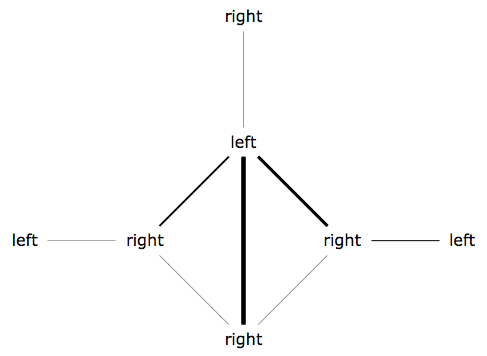
\includegraphics[width=8cm, height=6cm]{taking-sides-graph.png}\\
%  \caption{Grafo extraído de \cite{malouf-taking_sides}. Os vértices são usuários e as arestas, citações entre eles. Arestas mais escuras indicam frequência de citação mais alta.}
%  \label{fig:malouf}
%\end{figure}


%Padrões de citação a \emph{sites} também foram investigados \cite{efron}. No artigo de Miles Efron, os experimentos envolvem os \emph{datasets} \textbf{Political-Orientation} e \textbf{Artists}. O primeiro é composto de artigos políticos Estadunidenses de Direita ou Esquerda e o segundo é composto de textos sobre artistas musicais, divididos entre as categorias Alternativo e Popular. As taxas de acerto relatadas para as aplicações de Naïve Bayes nestes corpora foram de, respectivamente, 64.71\% e 50.1\%. A fim de melhorar as taxas de acerto na classificação dos documentos, o artigo estima a perspectiva de cada um deles avaliando a probabilidade de que eles sejam co-citados, na Web, com documentos referência de cada perspectiva. Estes documentos de referência são agrupados em listas de URLs. Esta metodologia, aplicada a \textbf{Political-Orientation}, resultou em uma taxa de acerto de 94.1\%. Para \textbf{Artists}, a taxa de acerto máxima obtida foi de 88.84\%.

%Todos os artigos que propuseram metodologias para melhorar a classificação em corpora com vocabulários muito uniformes consideraram algum esquema de citação. Se o corpus for composto de documentos pouco citados na Web, o esquema do artigo de Miles Efron pode não trazer nenhuma melhoria significativa ao problema. Se os autores dos documentos não mencionarem significativamente um ao outro, como aconteceu nos estudos com o \emph{dataset} \textbf{Politics}, a metodologia explorada por Tony Mullen e Robert Malouf não é recomendada. Essa área de pesquisa, portanto, ainda tem alguns problemas em aberto - e, considerando que estes três artigos foram escritos há mais de quatro anos, ela não parece atrair muita atenção. A justificativa para isso, provavelmente, tem a ver com o fato de que uniformidade no vocabulário não é um problema tão comum em Mineração de Perspectiva. No \textbf{capítulo X}, técnicas envolvendo comparação entre documentos, que podem trazer benefícios à classificação de \emph{datasets} difíceis - e neste caso também se enquadram aqueles em que o vocabulário é mais uniforme -, serão discutidas.

\section{Conclusão}

Este capítulo apresentou duas hipóteses linguísticas assumidas por métodos baseados em frequências de palavras: 1) palavras específicas, denominadas \emph{banner words}, costumam ser utilizadas para defender perspectivas diferentes e 2) a quantidade de vezes que uma palavra é mencionada em um documento está diretamente relacionada com seu enfoque \cite{teubert2001}. Como consequência, esses métodos funcionam melhor em \emph{datasets} nos quais o emprego de palavras varia significativamente por perspectiva. %tão melhor quanto mais diferentes forem os empregos de palavras por perspectiva.

%ideia de que pessoas costumam utilizar palavras específicas, denominadas \emph{stigma words} ou \emph{banner words}, para defender perspectivas diferentes. O uso de classificadores baseados na presença ou frequência das palavras, portanto, costuma funcionar bem na identificação dessas perspectivas. Entretanto, em alguns casos, as construções do discurso refletem diferentes perspectivas melhor do que o uso de palavras específicas. Nestes casos, as taxas de acerto desses classificadores são menores do que o desejado. 

Para ilustrar a relação entre as palavras de dois \emph{datasets} e o desempenho desses métodos, experimentos com o modelo de tópicos L-LDA foram executados. A extração das dez palavras mais fortemente associadas a cada tópico conduziu à visualização parcial de como o vocabulário dos \emph{datasets} se agrupa em torno de suas diferentes perspectivas. A informação, apesar de subjetiva, auxilia na compreensão das taxas de acerto obtidas com um classificador Naïve Bayes padrão, aplicado aos dois corpora. Para o primeiro \emph{dataset}, as taxas de acerto obtidas foram mais altas, o que pode ser explicado por uma presença maior de \emph{banner words} em comparação com o segundo \emph{dataset}.

Métodos baseados em frequências de palavras foram explorados pela maioria dos trabalhos revisados para esta monografia - mesmo fazendo parte de metodologias mais complexas. Apesar de outros fatores contribuírem para o mau desempenho destes métodos, como um número muito pequeno de documentos no \emph{dataset}, é interessante investigar o vocabulário do corpus caso as taxas de acerto obtidas estejam aquém do desejado. O uso de um modelo de tópicos L-LDA, agrupando palavras por perspectiva, é útil para compreender como os autores dos documentos se expressam. Se as palavras são empregadas de modo muito parecido por todas as perspectivas, isto justifica, ainda que em parte, o mau desempenho obtido.

% voa relação entre as palavras contidas em dois \emph{datasets} e suas diferentes perspectivas. No primeiro \emph{dataset}, as palavras extraídas para cada perspectiva se relacionam, semanticamente, melhor com a perspectiva em si do que no segundo \emph{dataset}. Neste último, palavras genéricas, como artigos e conjunções, se associam muito fortemente a todas as perspectivas, colaborando para uma uniformização do vocabulário. Isto explica, ainda que não seja trivial avaliar o quanto, as taxas de acerto mais altas obtidas com um Naïve Bayes no primeiro \emph{dataset}.

%Por fim, este capítulo também revisa artigos que discutem a questão do vocabulário do corpus. Estes artigos propõem metodologias para melhorar a classificação em \emph{datasets} cujo vocabulário é considerado muito uniforme - todas baseadas em algum esquema de citação a documentos. A questão do vocabulário do corpus é pouco discutida na literatura; provavelmente porque o problema é pouco comum e porque outros métodos, mais genéricos para \emph{datasets} difíceis de classificar, têm sido mais estudados.
 
%o primeiro \emph{dataset}, os artigos estão escritos sob uma das seguintes perspectivas: pró-Palestina ou pró-Israel. Por conta disso, o tópico \emph{pal} foi atribuído a todos os documentos pró-Palestina e o tópico \emph{isr}, a todos os pró-Israel. Estes tópicos facilitam a visualização das palavras mais fortemente associadas a cada uma das duas perspectivas, de acordo com o vocabulário empregado nos artigos. Um terceiro tópico, \emph{gen}, foi atribuído a todos os documentos, a fim de capturar as palavras que co-ocorrem neles independentemente de suas perspectivas. Após a execução do modelo, as 100 palavras mais fortemente associadas a cada um dos 3 tópicos foram coletadas. 35\% das associadas a \emph{isr} não estão presentes no conjunto recolhido para \emph{gen}. Para \emph{pal}, essa percentagem cai para 29\%. Por fim, 32\% das palavras mais fortemente associadas a \emph{isr} não fazem parte das 100 palavras mais fortemente associadas a \emph{pal} e vice-versa. Essas percentagens indicam que os autores dos documentos pró-Israel utilizam um vocabulário ligeiramente mais específico, na defesa de seus pontos de vista, do que os autores pró-Palestina. É importante ressaltar que nenhuma palavra foi filtrada na análise - ou seja, termos muito frequentes como \emph{the}, \emph{of} e \emph{and}, comumente extraídos dos \emph{datasets} antes da etapa de classificação, estavam presentes nos documentos processados pelo L-LDA.    

%Palavras associadas a \emph{isr} que não foram associadas a \emph{gen}
%['arafat', 'be', 'some', 'roadmap', 'us', 'yet', 'out', 'sharon', 'ariel', 'support', 'three', 'bush', 'palestine', 'new', 'terrorism', 'leader', 'then', 'jewish', 'after', 'arab', 'leadership', 'plan', 'president', 'than', 'bank', 'prime', 'regarding', 'like', 'could', 'violence', 'against', 'while', 'time', 'american', 'first']

%Palavras associadas a \emph{pal} que não foram associadas a \emph{gen}
%['then', 'some', 'authority', 'against', 'occupied', 'negotiations', 'occupation', 'sharon', 'united', 'end', 'way', 'palestine', 'international', 'be', 'after', 'plan', 'president', 'law', 'those', 'prime', 'land', 'i', 'violence', 'us', 'q', 'while', 'time', 'situation', 'first']

%Palavras associadas a \emph{pal} que não foram associadas a \emph{isr}
%['because', 'people', 'authority', 'states', 'right', 'occupied', 'any', 'negotiations', 'occupation', 'what', 'united', 'end', 'also', 'been', 'their', 'other', 'way', 'international', 'law', 'do', 'which', 'government', 'very', 'they', 'now', 'those', 'about', 'land', 'these', 'q', 'i', 'situation']

%Palavras associadas a \emph{isr} que não foram associadas a \emph{pal}
%['arafat', 'into', 'settlements', 'years', 'yet', 'out', 'even', 'would', 'ariel', 'west', 'support', 'three', 'bush', 'gaza', 'new', 'terrorism', 'leader', 'we', 'jewish', 'arab', 'most', 'leadership', 'minister', 'roadmap', 'than', 'bank', 'both', 'regarding', 'like', 'could', 'war', 'american']
%\textbf{As palavras estão ordenadas de acordo com a força da associação com cada um dos tópicos}


%\textbf{Lista de palavras e desempenho. Imagens e Tabelas.}

%Dado que em boa parte dos artigos estudados neste projeto, como \cite{lin-et-al2006} e \cite{klebanov}, atinge-se taxas de acerto superiores a 80\% com classificadores baseados em frequência de palavras, conclui-se que a mineração de perspectivas em discussões, artigos opinativos e debates requer metodologias diferentes, a depender de como as palavras foram escolhidas pelos autores dos documentos. %Nos debates estudados por \cite{hirst-et-al}, expressões de ataque e defesa são mais frequentes do que \emph{stigma words} e, como o método empregado no artigo foi um SVM treinado com frequências de palavras, observou-se que a classificação obtida para os lados do debate não refletia as perspectivas \emph{liberal} ou \emph{conservadora} - mas sim os lados \emph{oposição} (expressões de ataque) e \emph{situação} (expressões de defesa). 
%Estes estudos indicam a possibilidade de que, em debates e discussões nos quais há uma homogeneização do vocabulário empregado - o que pode acontecer quando todos os lados utilizam, em proporções similares, tanto expressões de ataque quanto de defesa -, classificadores baseados exclusivamente nas palavras utilizadas e/ou em suas frequências apresentarão má performance.

%A avaliação do desempenho desses classificadores\footnote{\textbf{SVMs e Naive Bayes padrão; LSPM}} nos \emph{datasets} estudados revela que artigos opinativos e notícias consolidaram perspectivas, através da escolha do vocabulário utilizado, melhor do que debates. Apesar disso, uma generalização neste sentido, restringindo o uso desses classificadores a artigos e notícias, não é recomendada por falta de indicativos linguísticos que comprovem essa tendência. Uma estratégia que pode ajudar na escolha ou descarte de um classificador desse tipo é uma análise das palavras que estão contidas nos documentos.

%\textbf{mostrar as percentagens prum dataset onde a linguagem eh mais uniforme. discutir.} 
%Explicar q isso nunca foi feito e q pessoas q ncontraram merda com essa feature fizeram outras coisas. descrever essas coisas.

%Estas hipóteses ilustram  
%Como indica \cite{}: 

%\textbf{MODO RASCUNHO AINDA}

%Explicar que uma diferença fundamental notada entre os datasets observados diz respeito à formalidade da linguagem empregada nos documentos. Enquanto alguns datasets utilizam documentos provenientes de meios onde a norma culta da linguagem impera, e uma revisão ortográfica é utilizada, outros são carregados de gírias, expressões e abreviações típicas da linguagem da Internet e contêm, eventualmente, grafias erradas para uma mesma palavra. <Dar exemplos textuais. Mostrar uma tabelinha, algo assim, indicando o volume de datasets com linguagem informal nos documentos estudados.> 

%A linguagem informal pode criar alguns desafios para a Mineração de Perspectiva [FECHAR O PROBLEMA EM: IDENTIFICAÇÃO DA PERSPECTIVA PRESENTE EM UM DOCUMENTO], especificamente no que diz respeito ao pré-processamento dos documentos e à escolha do método empregado. No pré-processamento, como indicado em (aaai-politics.pdf e 10.1.1.138.7160.pdf), a correção gramatical das palavras é bastante indicada. Com uma única versão de grafia para cada palavra (a correta), diminui-se a quantidade de ruído que grafias erradas podem causar na classificação.

%Uma característica dos datasets que deveria ser considerada sempre antes de se escolher o método utilizado - mas não é prática entre as pessoas que estudam perspective mining - é a frequência das palavras nos documentos do dataset. Se o léxico empregado pelos autores dos textos muda sensivelmente a depender de sua ideologia/perspectiva defendida/ponto de vista, é possível resolver o problema utilizando classificadores que usam essa frequencia como feature. GASTE TEMPO DANDO ALGUNS EXEMPLOS.  Em datasets informais, entretanto, como aponta Efron, a linguagem empregada por todos os lados da discussão pode ser basicamente a mesma: termos com forte carga de polaridade e gírias/jargões comuns na discussão [EXEMPLO]. Neste caso, é preciso utilizar métodos que utilizem mecanismos mais rebuscados do que a simples frequência/presença das palavras no texto. Alguns autores utilizam métodos mais gramaticais para lidar com datasets informais, como é o caso de , BLE e BLI. Os 2 primeiros criam o conceito de Opinion Frame (DEFINIR O CONCEITO). No primeiro caso, a ideia é associar corretamente opiniões a alvos, e associar alvos iguais utilizando técnicas de co-referência. Segundo Wiebe et al. (pegar a citação corretamente), ter as targets associadas, com as opiniões próximas, é uma boa forma de entender o overall de opiniões de um documento. A estratégia é uma alternativa possível para documentos em que as perspectivas estão muito associadas à linguagem opinativa, e onde essa linguagem é comum para todos os lados. Infelizmente, os resultados alcançados indicam que a tarefa não é trivial: blablablablababla (resolver coreferencia pra linkar targets não é tão simples assim => e dê exemplo). 

%uma diferença fundamental notada entre os \emph{datasets} observados diz respeito à formalidade da linguagem empregada nos documentos. Enquanto alguns datasets utilizam documentos provenientes de meios onde a norma culta da linguagem impera, e uma revisão ortográfica é utilizada, outros são carregados de gírias, expressões e abreviações típicas da linguagem da Internet e contêm, eventualmente, grafias erradas para uma mesma palavra. <Dar exemplos textuais. Mostrar uma tabelinha, algo assim, indicando o volume de datasets com linguagem informal nos documentos estudados.> 

\chapter{Metodologias que usam informação extra-documento}

\section{Concordância e discordância entre documentos}
  \textbf{Falar do Get Out the Vote e artigos que seguem a linha}

\section{Meta-informações sobre os autores}

\chapter{Metodologias que usam relações intra-documento}

\textbf{Falar de targets, uso de dicionários de polaridade, limitações importantes}

\chapter{Estudo de caso: Eleições 2010}

\chapter{Trabalhos relacionados}

\chapter{Conclusão}
\label{conclusoes}

Com a disseminação da Web, a elaboração e disseminação de textos carregados com um ponto de vista se popularizou. Não se tratam de documentos que trazem opiniões pontuais a respeito de um único objeto, como um filme ou um livro, mas sim a exposição de argumentos e ideias que, unidos, transmitem a defesa de uma posição a respeito de um certo tema. Enquanto opiniões envolvem um léxico mais restrito, composto de termos como \emph{bom} ou \emph{chato}, as palavras utilizadas na expressão de pontos de vista variam bastante de um tema para outro. Isto dificulta a construção de um conjunto de treinamento que se adeque bem a uma gama variada de temas e é, possivelmente, o principal motivo pelo qual ainda não foi desenvolvida nenhuma ferramenta voltada para pontos de vista genérica para \emph{qualquer tema}. 

Ainda assim, a demanda por entender como as pessoas se posicionam ideologicamente - e em larga escala - existe, e tem fomentado um número crescente de estudos voltados para temáticas específicas. Os artigos revisados no Capítulo \ref{chap3} indicam que a classificação por ponto de vista é mais aplicada a \emph{datasets} que envolvem posicionamentos políticos e temáticas polêmicas, como pena de morte. A leitura da \emph{survey} de Pang e Lee e de alguns artigos sugere, por sua vez, que a classificação por opiniões tem sido mais explorada em \emph{datasets} que envolvem produtos ou serviços \cite{omsa, thumbs-up, peanut-gallery}.

A revisão apresentada no Capítulo \ref{chap3}, além de indicar preferências temáticas na área, também aponta algumas predileções metodológicas. A maioria dos trabalhos classifica os documentos com um Naïve Bayes ou um SVM. Em boa parte dos casos, essa classificação explora apenas as diferentes contagens de palavras nos documentos. Alguns outros artigos exploram propriedades sintáticas ou semânticas dos \emph{datasets} analisados. Outros, por fim, consideram as interações entre os documentos na determinação de seus pontos de vista. A contagem de palavras, simples de ser computada em qualquer língua, foi a característica mais estudada pelos trabalhos revisados - ainda que não tenha recebido destaque em todos eles. Em boa parte dos casos, seu uso exclusivo já é suficiente para uma boa classificação. Em alguns outros, o uso de outras estratégias, mais complexas, foi fundamental para a melhoria na classificação. Diante disso, recomenda-se, inicialmente, para o problema de classificação por ponto de vista, o uso \emph{exclusivo} de contagens de palavras. Se os resultados obtidos não forem satisfatórios, recomenda-se a escolha de um subconjunto ótimo de palavras, como indica o trabalho de Durant e Smith \cite{durant-smith}. Apenas se não houver melhorias significativas, recomenda-se o uso de outras características, um pré-processamento de documentos mais refinado ou a investigação das interações entre os documentos. Essas recomendações, portanto, partem das ideias mais simples para as mais complexas, evitando esforços desnecessários. 
%INTERNACIONALIZÁVEEEEEL!!
%o uso de um pré-processamento mais refinado dos documentos ou 

%Contagens de palavras foram exploradas por muitos artigos, como características diferenciadoras de pontos de vista. De fato, a classificação baseada em contagens de palavras, ou em alguma de suas variações (como a presença/ausência de palavras), assume uma hipótese defendida em estudos de Linguística de corpus: a quantidade de vezes que uma palavra é mencionada em um documento (sua contagem) está diretamente relacionada a quais ideias ele destaca \cite{teubert}. Como consequência, ela funciona melhor em \emph{datasets} nos quais o emprego de palavras varia significativamente por perspectiva. A fim de investigar como o uso de palavras, refletido em suas contagens, se associa ao desempenho da classificação, o Capítulo \ref{chap3} apresenta alguns experimentos neste sentido. Dois corpora são classificados com um Naïve Bayes baseado em contagens de palavras. Via validação cruzada, as taxas de acerto obtidas foram, respectivamente, de 86.22\% e 54.01\%. Isso significa que, no primeiro corpus, as contagens de palavras foram suficientes para identificar corretamente a classe dos documentos de forma satisfatória; no segundo corpus, tem-se o caso contrário. Em outras palavras, isso significa que, no primeiro corpus, o emprego de palavras varia significativamente por perspectiva; no segundo, não. 

%A fim de verificar quais palavras foram mais enfocadas por cada ponto de vista, ampliando a compreensão dos resultados obtidos com o Naïve Bayes, foram feitos experimentos com o modelo L-LDA\footnote{O L-LDA é apresentado no Capítulo \ref{basicos}.}. O modelo associa palavras a tópicos, facilitando a visualização de quais são mais relevantes para cada um deles. Nesses experimentos, cada perspectiva de cada \emph{dataset} corresponde a um tópico, e um último tópico, neutro, é associado a todos os documentos. A finalidade do tópico neutro é filtrar palavras muito comuns em cada corpus, independentemente de perspectiva. Com isso, evidencia-se quais palavras receberam mais destaque por cada perspectiva. Selecionando-se as dez palavras mais frequentemente associadas a cada perspectiva, já é possível visualizar que, no primeiro corpus, perspectivas diferentes enfatizam ideias mais distintas do que no segundo corpus. Isso amplia a compreensão das classificações feitas com o Naïve Bayes, apresentando cenários em que o uso exclusivo de contagens de palavras é ou não suficiente para uma boa classificação. É importante frisar que não se encontrou nenhum outro trabalho que faça uso de um L-LDA para compreender, ainda que parcialmente, como certos termos são enfocados por diferentes perspectivas.

Aproveitando as revisões e análises apresentadas no Capítulo \ref{chap3}, decidiu-se fazer um estudo de caso envolvendo um \emph{dataset} brasileiro. É válido ressaltar que não foi encontrado nenhum outro trabalho que classifique documentos, escritos em português do Brasil, de acordo com seus pontos de vista. Considerando que 2010 é ano de eleições presidenciais no Brasil, a abundância de artigos que carregam pontos de vista típicos da oposição e da situação foi explorada. Foi construído um corpus sobre o atual governo e as eleições, composto de material coletado em colunas, \emph{sites} e \emph{blogs} mantidos por jornalistas de notoriedade nacional. Em seguida, esse corpus foi dividido entre os pontos de vista pró-situação e pró-oposição, e foi classificado com um Naïve Bayes. As características dos documentos exploradas por esse classificador foram suas contagens de palavras. Os resultados obtidos com essa metodologia foram muito positivos: a taxa de acerto, em particular, foi de 89.43\%. Isso significa que esses jornalistas consolidam suas perspectivas sobre a política brasileira já nas palavras que destacam. De fato, alguns trechos elencados no Capítulo \ref{estudo}, no qual o estudo é apresentado, sugerem que seus pontos de vista são defendidos com muita veemência. 

Esse estudo de caso também investiga quais palavras receberam mais destaque por cada ponto de vista. A análise com um L-LDA, associando cada ponto de vista a um tópico e um tópico neutro a todos os documentos, indica que os jornalistas pró-situação dão mais ênfase ao candidato de oposição José Serra do que os pró-oposição. Esses últimos, por sua vez, dão maior destaque ao presidente Lula e à sua candidata, Dilma Rousseff - ambos correspondem à situação. Isso sugere que os jornalistas enfatizam o ataque aos candidatos que se opõem, ideologicamente, aos pontos de vista que eles defendem. Isso reforça a ideia, empiricamente observável, de que a defesa de um posicionamento, muitas vezes, compreende o ataque a posicionamentos opostos, como sugerem Somasundaran e Wiebe em seu trabalho sobre debates \emph{online} \cite{wiebe}.  
%, assim como no Capítulo \ref{chap3},
%cado de forma semelhante àquela do Capítulo \ref{chap3}, 

\section{Dificuldades encontradas}

A classificação de documentos de acordo com seus pontos de vista sobre um tema é um problema relativamente novo. De fato, ele só foi estabelecido como sub-área da Mineração de Opinião em 2008, na \emph{survey} de Pang e Lee. Por este motivo, para entender melhor o problema, foi necessário buscar artigos em diversas conferências que envolviam a área de Mineração de Opinião. A filtragem de quais resultados realmente tinham a ver com o tema dessa monografia não foi exatamente difícil, mas envolveu um trabalho manual considerável. Para o estudo de caso, a extração, filtragem e padronização dos documentos que compõem o corpus também envolveu algum trabalho manual. Embora essas tarefas tenham sido realizadas de forma automatizada, a construção dos \emph{scripts} dependia da compreensão de como o conteúdo estava disposto em cada veículo.  

\section{Trabalhos futuros}

Futuramente, pretende-se estender o estudo de caso do Capítulo \ref{estudo} a textos políticos escritos por cidadãos comuns em seus \emph{blogs}, o que pode contribuir positivamente para a compreensão de como o brasileiro se posiciona politicamente na Web. Além disso, o estudo também deve ser ampliado para identificar os pontos de vista contidos nos comentários feitos aos artigos do corpus, em seus \emph{blogs}, \emph{sites} e colunas, a fim de se avaliar como eles refletem o posicionamento dos leitores em relação àquilo que leram. Este tipo de análise pode ajudar a compreender o impacto destes artigos em seus leitores e a formação de posicionamentos na mídia brasileira \emph{online}. Caso essas tarefas de classificação não sejam bem resolvidas com o uso exclusivo de contagens de palavras, esforços direcionados na busca de características mais complexas, envolvendo aspectos sintáticos/semânticos dos documentos, devem ser feitos. É válido ressaltar que isso provavelmente implicaria no desenvolvimento de ferramentas gramaticais de apoio, voltadas para a língua portuguesa.



\appendix

\chapter{Teorema de Bayes e notações}

A Estatística se alia à Teoria da Probabilidade para estimar e analisar a ocorrência de eventos, como \emph{Ganho de cem reais em sorteio} ou \emph{Chuva ao meio-dia}. Dados dois eventos \emph{A} e \emph{B}, temos que a probabilidade \emph{a priori} de \emph{A} acontecer \textbf{ignora} a ocorrência do evento \emph{B}. Essa probabilidade é representada pela notação \ensuremath{P(A)}. Analogamente, para o evento \emph{B}, tem-se \ensuremath{P(B)}. Na prática sabe-se, intuitivamente, que a ocorrência de determinados eventos interfere no acontecimento de outros. Se às onze e meia da manhã observa-se o evento \emph{Céu nublado}, a probabilidade do evento \emph{Chuva ao meio-dia} ocorrer pode diferir daquela que ignora esse primeiro evento. Neste sentido, a probabilidade de um evento \emph{A} ocorrer \emph{dado} que \emph{B} ocorreu recebe o nome de probabilidade \emph{a posteriori} de \emph{A} condicional a \emph{B}, e é denotada por \ensuremath{P(A\mbox{ }|\mbox{ }B)}. Analogamente, tem-se \ensuremath{P(B\mbox{ }|\mbox{ }A)}. O Teorema de Bayes correlaciona essas probabilidades da seguinte forma 

\begin{equation}
\label{bayes-apendice}
\ensuremath{P(A\mbox{ }|\mbox{ }B) = \frac{P(B\mbox{ }|\mbox{ }A)P(A)}{P(B)}} 
\end{equation}

O classificador Naïve Bayes se baseia em uma aplicação direta do Teorema de Bayes. Dados os eventos \emph{Obtenção de um documento x} e \emph{Obtenção de uma classe y}, o classificador deve estimar a ocorrência do segundo evento assumindo que o primeiro já ocorreu.   



\bibliography{monografia}

\end{document}

